The development process of any constitutive model involves testing of the individual components which make up the model.

\begin{wrapfigure}{r}{0.45\textwidth}
 \includegraphics[width=0.45\textwidth]{images/Result_correspondence_matrix.pdf}
 \caption{Testing the Correspondence Matrix subroutine.}
  \label{Correspondence_matrix_program}
\end{wrapfigure}



Model study can be further divided into ``component testing" where we test individual components of the model and ``model testing" where we test the entire model.

\section{Model Component testing}

\subsection{Testing Correspondence Matrix subroutine.}

The subroutine for generating the correspondence matrix was written inside the framework of the DAMASK. It utilizes many intrinsic components within the DAMASK such as:

\begin{itemize}
    \item Schmid Matrix.
    \item Generation of Normal Vector and Direction vector for different twin system
    \item Generation of Characteristic Shear for different twinning modes and also for different c/a ratios.
\end{itemize}

A new function was also introduced. This function generates the re-indexation matrix from the normal vector.

The correspondence matrix subroutine generates the correspondence matrix for different types of twins and HCP metals with different c/a ratios.

The complete program to generate the correspondence matrix is given in Appendix \ref{Appendix:Correspondence_matrix}

The figure \ref{Correspondence_matrix_program} is the result from the program used to generate the correspondence matrix.


\subsection{Testing the reorientation in the deformation kinematics.}
The multiplicative decomposition is done such that the current crystallographic orientation $O$ can then always be calculated from elastic deformation gradient $F_e$ through a polar decomposition 
\begin{equation*}
    F_e = O^T U
\end{equation*}
 where $U$ is the right stretch tensor.

 We use this result to verify that the pre-multiplication of correspondence matrix will result in the reorientation of twinned lattice in the single constituent kinematics formulation of the DAMASK.
\subsubsection{Brief summary of the code to test reorientation:}
First, the code defines parameters such as twin direction, habit plane normal, material properties, and initial Euler angles. These values are then used to calculate the norm of the twin direction and plane normal, unit vectors, and characteristic shear for extension twinning. The initial orientation of the crystal is defined using Euler angles. The twinning operation is applied by multiplying the deformation gradient with the correspondence matrix. Polar decomposition of the final deformation gradient is performed to separate the rotation and stretching components. Finally, the code calculates the disorientation angle between the initial and final crystal orientations, which quantifies the amount of rotation caused by twinning.

 The verification is done using a python script given in Appendix \ref{Appendix:Correspondence_matrix}. The figure \ref{Reorientation_test} shows the result of the python script.

 \begin{figure}[H]
    \centering
    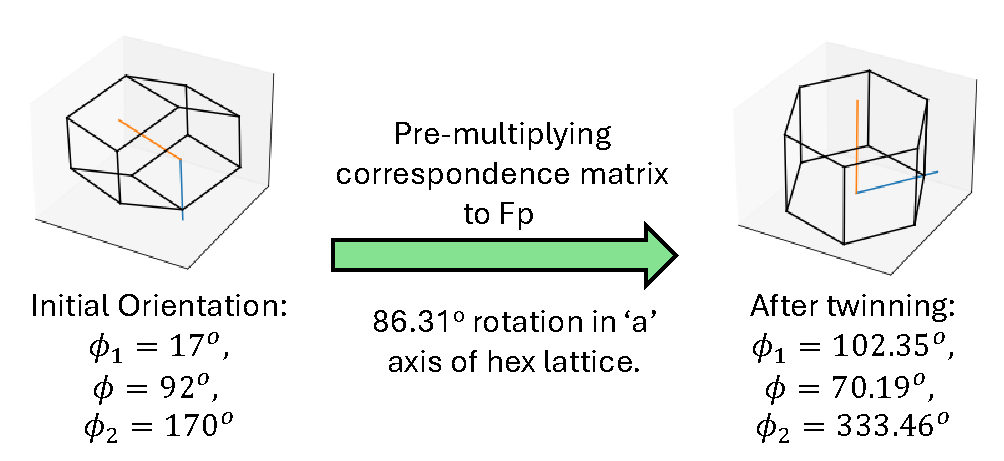
\includegraphics[width=0.7\textwidth]{images/Reorientation_Test.pdf}
    \caption{Reorientation test.}
    \label{Reorientation_test}
 \end{figure}

\section{Model Testing}

For testing the entire model, it is necessary to run a complete DAMASK simulation. In this section DAMASK simulation workflow is briefly discussed.

\subsection{The DAMASK simulation procedure.}

A typical DAMASK simulation procedure consist of preprocessing tasks to create the input files for running the simulation and postprocessing tasks to read and analyze the output file from the simulation.

Figure \ref{DAMASK_workflow} shows the DAMASK simulation procedure.

\begin{figure}[H]
    \centering
    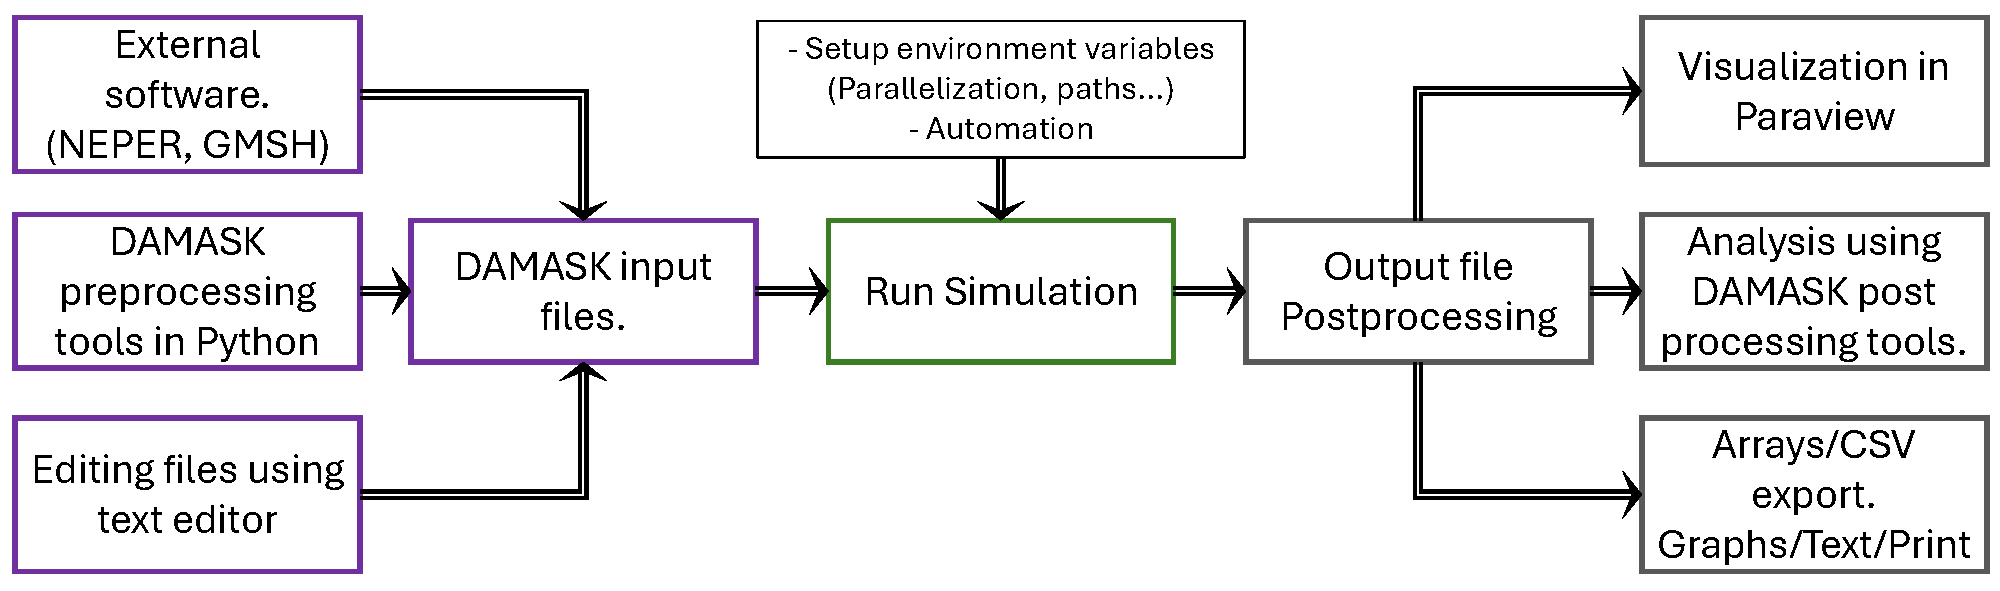
\includegraphics[width=\textwidth]{images/DAMASK_workflow.pdf}
    \caption{Flow chart of DAMASK Simulation Procedure.}
    \label{DAMASK_workflow}
\end{figure}

\subsubsection{Preprocessing}
Preprocessing involves generation of 3 input files:
\begin{enumerate}
\item Geometry file (*.vti for FFT solver or *.msh for FEM solver) \\ Geomtery file has the details of the Representative Volume Element(RVE) which contains the details about grain size, shape, volume etc.\\
Geometry file can be generated using DAMASK preprocessing tools in Python or using external software like NEPER or GMSH.
\item \{Material\}.yaml file: \\ Material file has the details of microstructural parameters like elastic constants, lattice parameters, the orientation of each grain in the RVE. It also has details about the constitutive law used and the parameters used in the constitutive law like slip parameters, twin parameters, etc. \\
\{Material\}.yaml file can be generated using DAMASK preprocessing tools, it can also be edited using a text editor.
\item \{Load\}.yaml file: \\ Load file has the details of boundary conditions and discretization which can be given in steps.
The displacement boundary condition can be defined in terms of $\Dot{F}$ or $L$ or $F$ (rate of deformation gradient, velocity gradient or deformation gradient) and load boundary condition can be defined in terms on $\Dot{P}$(rate of First-Piola-Kirchoff-Stress) or P (PK1).\\
\{Load\}.yaml file can be generated using DAMASK preprocessing tools and it can be edited using a text editor.
\end{enumerate}

\subsubsection{Simulation}
Before running a simulation the environment can be set for DAMASK by running 
\begin{lstlisting}[language=bash, basicstyle=\small\ttfamily, frame=single]
source ./{DAMASK_source_folder_path}/env/DAMASK.sh
\end{lstlisting}

DAMASK has gives choice between FFT and FEM solvers which are part of DAMASK. Simulations can also be run in MSC MARC solver. For our work we primarily use FFT solver or ``DAMASK\_grid".

\subsubsection{Postprocessing}
The data from the DAMASK simulation will be stored in HDF5 (Hierarchical Data File) file.  Data in the HDF5 output files has to be processed for further analysis or visualization. DAMASK provides postprocessing tools in Python to make manipulate and process the data in HDF5 files.



\subsection{Bycrystal Representative Volume Element.}

For testing our mechanical twinning model, we employ a 2-dimensional bicrystal RVE containing a hard matrix phase and a soft inclusion phase. The hard surrounding crystal or ``matrix" is oriented such that it has a higher critical resolved shear stress for activating twinning, while the soft inclusion is more amenable to mechanical twinning. This offers us simple test case consisting of two grains with a grain boundary. The RVE is of dimension 100$\mu$mx100$\mu$m and it is discretized to 64x64 FFT grid elements. This simple RVE is used to test our discrete twinning model.

\begin{figure}[H]
    \centering
    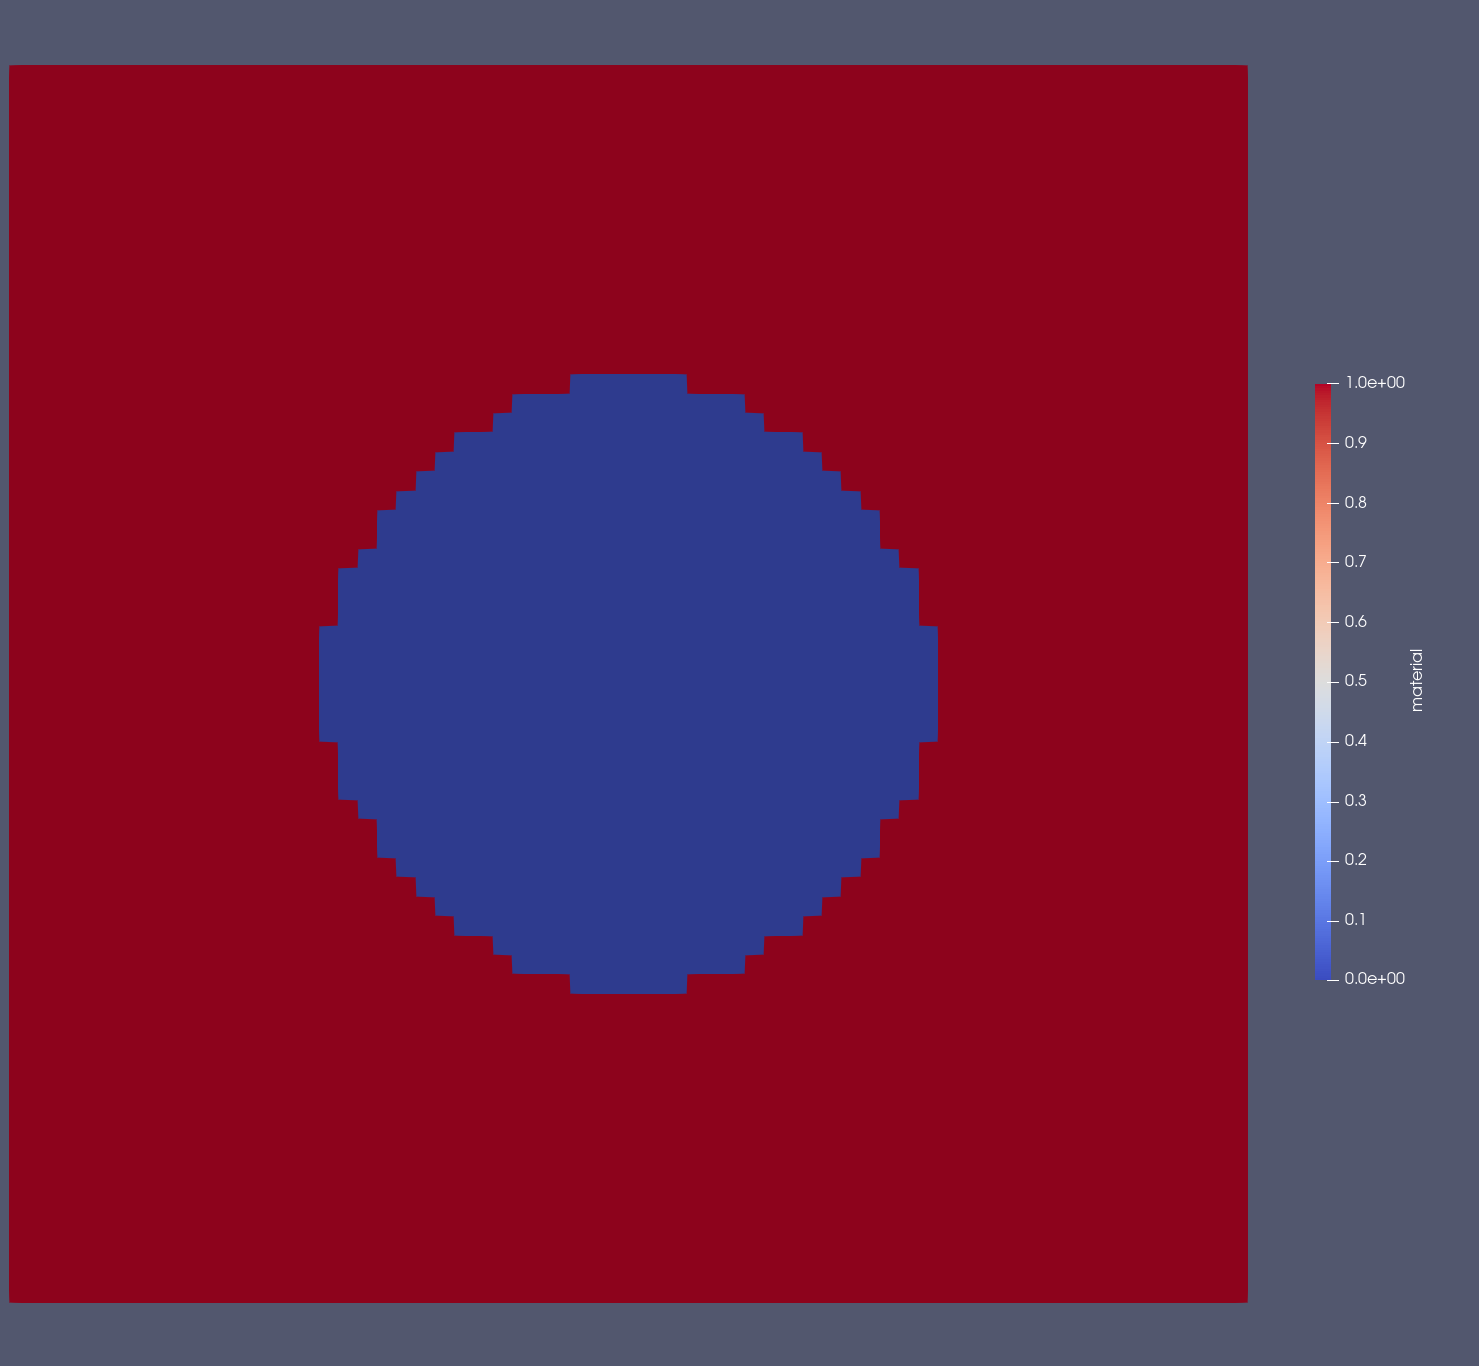
\includegraphics[width=0.4\textwidth]{images/Bycrystal_RVE.png}
    \caption{Bicrystal Representative Volume Element.}
    \label{fig:Bycrystal RVE.}
\end{figure}

%Schmid Factor for twinning

%Boundary Condition
%Boundary condition is given for this test case as:


\subsection{Test for nucleation.}

\begin{figure}[H]
    \centering
    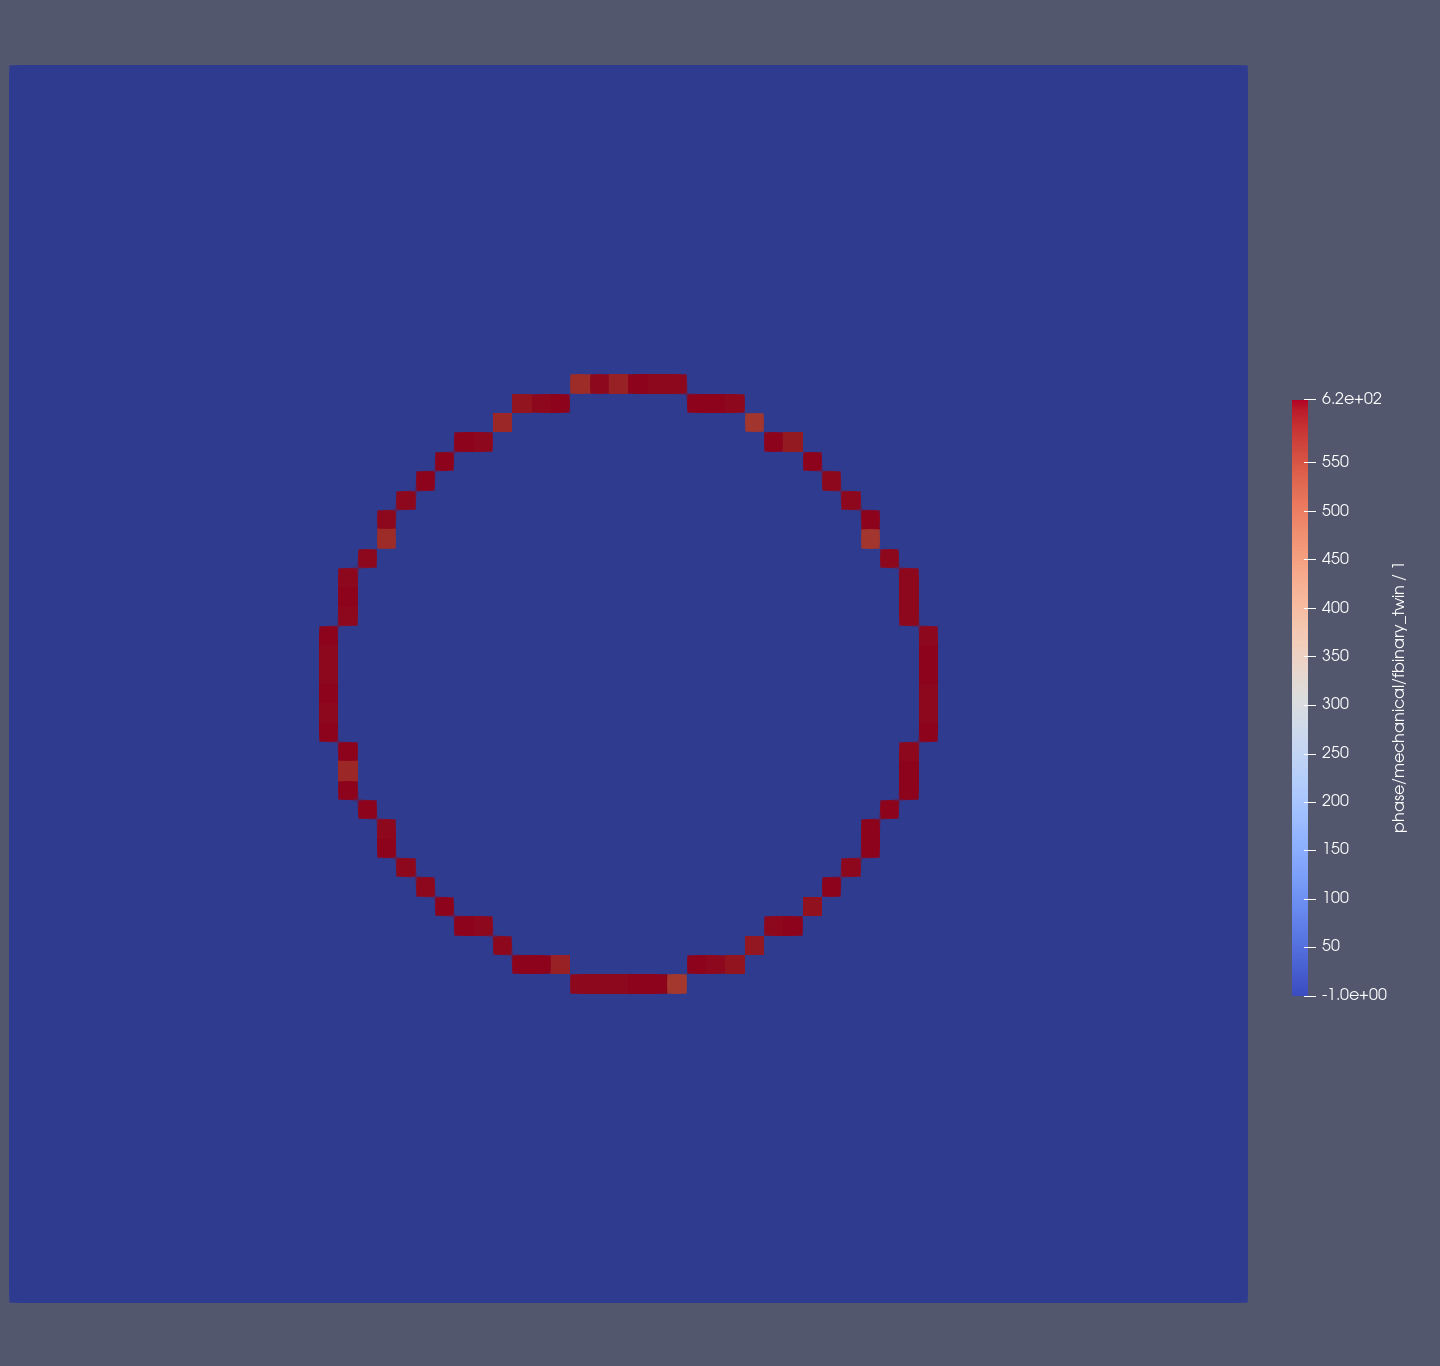
\includegraphics[width=0.4\textwidth]{images/Grain boundray identification test.png}
    \caption{Selection of grain boundary elements for nucleation.}
    \label{fig:Selection of grain boundary elements.}
\end{figure}

The nucleation of the twins are assumed to occur at the grain boundaries. Grain boundary is the surface at which single crystals having different orientations meet each other. The nucleation code identifies the neighbours and if the two neighbouring elements have different orientations, then we consider the elements to be at the grain boundary. Grain boundary elements are sampled for nucleation. We take a bicrystal RVE to test the nucleation.

The figure \ref{fig:Selection of grain boundary elements.} shows the bicrystal RVE which shows the grain boundary elements which are identified as potential nucleation region.

\subsection{Test for growth.}
For testing the growth behavior, we consider the same program used for nucleation in addition with program for growth, as the growth process involves selective random sampling of the neighboring voxels/elements that are adjacent to twinned regions. Therefore, the growth process follows after the nucleation events. To test the growth behavior, we employ a bicrystal representative volume element (RVE). The image below illustrates the growth and band thickening of twins, which propagates from one grain boundary to another grain boundary. In this image the bycrystal RVE is superimposed on the simulation output which shows the variation of the discrete twinning variable "f\_binary"

\begin{figure}[H]
    \centering
    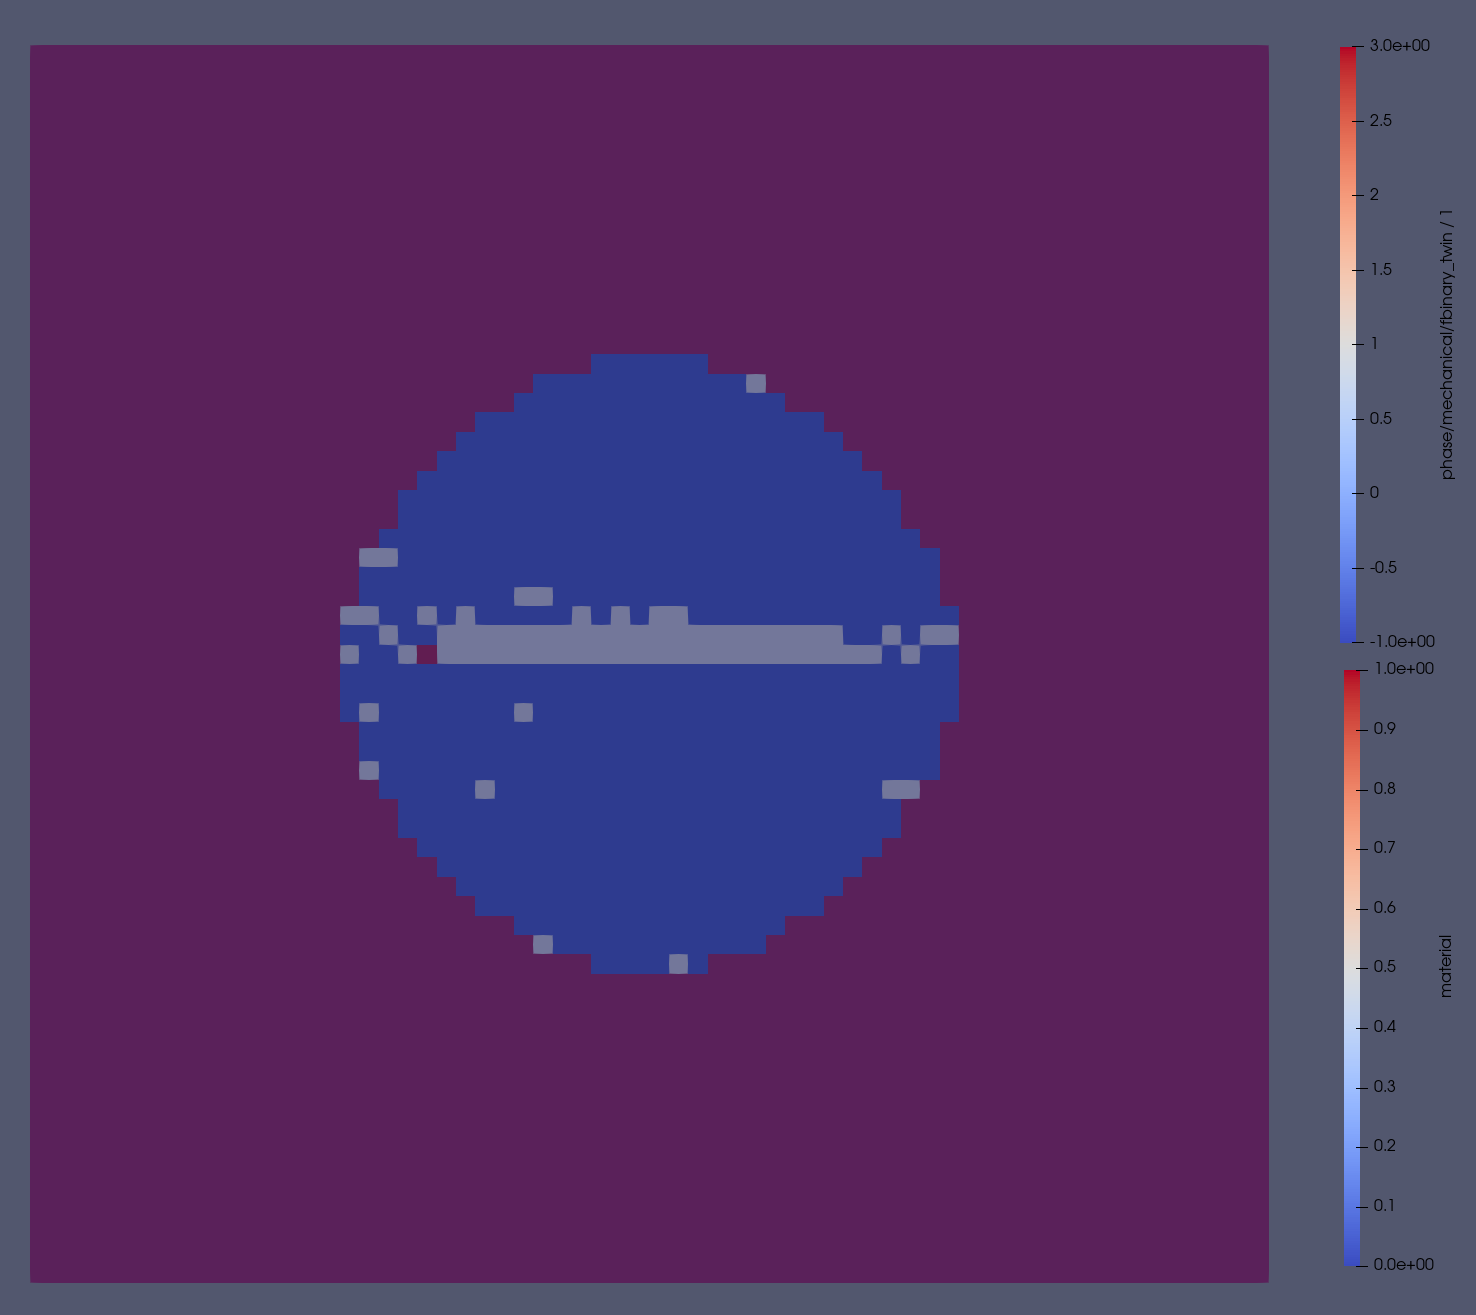
\includegraphics[width=0.4\textwidth]{images/Growth.png}
    \caption{Testing the program for growth.}
    \label{fig:Selection of neighbour elements for growth.}
\end{figure}